\documentclass[border=5pt]{standalone}
\usepackage[utf8]{inputenc}
\usepackage[T1]{fontenc}
\usepackage{tikz}
\usetikzlibrary{shapes.geometric,arrows.meta,positioning,calc}

\definecolor{convcolor}{RGB}{100,149,237}
\definecolor{lstmcolor}{RGB}{255,165,0}
\definecolor{attncolor}{RGB}{147,112,219}
\definecolor{fccolor}{RGB}{60,179,113}
\definecolor{ragcolor}{RGB}{234,67,53}

\begin{document}
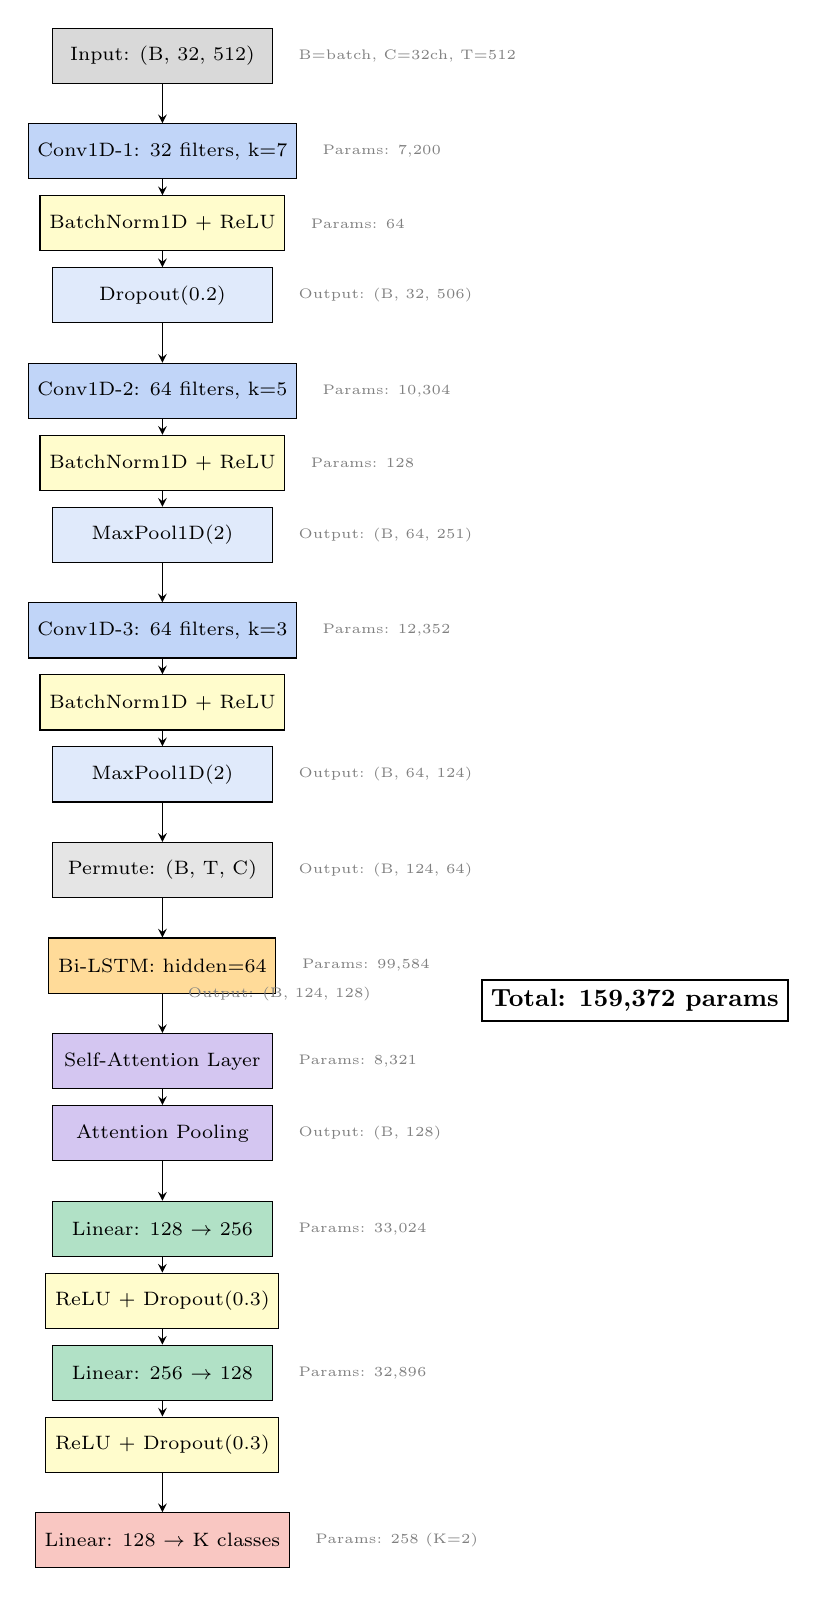
\begin{tikzpicture}[
    node distance=0.3cm,
    layer/.style={rectangle, draw, minimum width=2.8cm, minimum height=0.7cm, font=\scriptsize, text centered},
    input/.style={layer, fill=gray!30},
    conv/.style={layer, fill=convcolor!40},
    pool/.style={layer, fill=convcolor!20},
    lstm/.style={layer, fill=lstmcolor!40},
    attn/.style={layer, fill=attncolor!40},
    fc/.style={layer, fill=fccolor!40},
    output/.style={layer, fill=ragcolor!30},
    params/.style={font=\tiny, text=gray},
    arrow/.style={->,>=stealth}
]

% Input
\node[input] (input) {Input: (B, 32, 512)};
\node[params, right=0.2cm of input] {B=batch, C=32ch, T=512};

% Conv Block 1
\node[conv, below=0.5cm of input] (conv1) {Conv1D-1: 32 filters, k=7};
\node[params, right=0.2cm of conv1] {Params: 7,200};
\node[layer, fill=yellow!20, below=0.2cm of conv1] (bn1) {BatchNorm1D + ReLU};
\node[params, right=0.2cm of bn1] {Params: 64};
\node[pool, below=0.2cm of bn1] (drop1) {Dropout(0.2)};
\node[params, right=0.2cm of drop1] {Output: (B, 32, 506)};

% Conv Block 2
\node[conv, below=0.5cm of drop1] (conv2) {Conv1D-2: 64 filters, k=5};
\node[params, right=0.2cm of conv2] {Params: 10,304};
\node[layer, fill=yellow!20, below=0.2cm of conv2] (bn2) {BatchNorm1D + ReLU};
\node[params, right=0.2cm of bn2] {Params: 128};
\node[pool, below=0.2cm of bn2] (pool1) {MaxPool1D(2)};
\node[params, right=0.2cm of pool1] {Output: (B, 64, 251)};

% Conv Block 3
\node[conv, below=0.5cm of pool1] (conv3) {Conv1D-3: 64 filters, k=3};
\node[params, right=0.2cm of conv3] {Params: 12,352};
\node[layer, fill=yellow!20, below=0.2cm of conv3] (bn3) {BatchNorm1D + ReLU};
\node[pool, below=0.2cm of bn3] (pool2) {MaxPool1D(2)};
\node[params, right=0.2cm of pool2] {Output: (B, 64, 124)};

% Permute for LSTM
\node[layer, fill=gray!20, below=0.5cm of pool2] (permute) {Permute: (B, T, C)};
\node[params, right=0.2cm of permute] {Output: (B, 124, 64)};

% Bi-LSTM
\node[lstm, below=0.5cm of permute] (lstm1) {Bi-LSTM: hidden=64};
\node[params, right=0.2cm of lstm1] {Params: 99,584};
\node[params, below=0.1cm of lstm1, right=0.2cm] {Output: (B, 124, 128)};

% Attention
\node[attn, below=0.5cm of lstm1] (attn1) {Self-Attention Layer};
\node[params, right=0.2cm of attn1] {Params: 8,321};
\node[attn, below=0.2cm of attn1] (attn2) {Attention Pooling};
\node[params, right=0.2cm of attn2] {Output: (B, 128)};

% FC Layers
\node[fc, below=0.5cm of attn2] (fc1) {Linear: 128 $\rightarrow$ 256};
\node[params, right=0.2cm of fc1] {Params: 33,024};
\node[layer, fill=yellow!20, below=0.2cm of fc1] (relu1) {ReLU + Dropout(0.3)};
\node[fc, below=0.2cm of relu1] (fc2) {Linear: 256 $\rightarrow$ 128};
\node[params, right=0.2cm of fc2] {Params: 32,896};
\node[layer, fill=yellow!20, below=0.2cm of fc2] (relu2) {ReLU + Dropout(0.3)};

% Output
\node[output, below=0.5cm of relu2] (out) {Linear: 128 $\rightarrow$ K classes};
\node[params, right=0.2cm of out] {Params: 258 (K=2)};

% Arrows
\foreach \source/\dest in {input/conv1, conv1/bn1, bn1/drop1, drop1/conv2, conv2/bn2, bn2/pool1, pool1/conv3, conv3/bn3, bn3/pool2, pool2/permute, permute/lstm1, lstm1/attn1, attn1/attn2, attn2/fc1, fc1/relu1, relu1/fc2, fc2/relu2, relu2/out} {
    \draw[arrow] (\source) -- (\dest);
}

% Total params box
\node[draw, fill=white, thick, font=\small\bfseries] at (6,-12) {Total: 159,372 params};

\end{tikzpicture}
\end{document}
